\documentclass[12pt]{article}
\usepackage[paper=letterpaper,margin=1.5cm]{geometry}
\usepackage{amsmath}
\usepackage{amssymb}
\usepackage{amsfonts}
\usepackage{mathtools}
%\usepackage[utf8]{inputenc}
%\usepackage{newtxtext, newtxmath}
\usepackage{lmodern}     % set math font to Latin modern math
\usepackage[T1]{fontenc}
\renewcommand\rmdefault{ptm}
%\usepackage{enumitem}
\usepackage[shortlabels]{enumitem}
\usepackage{titling}
\usepackage{graphicx}
\usepackage[colorlinks=true]{hyperref}
\usepackage{setspace}
\usepackage{subfigure} 
\usepackage{braket}
\usepackage{color}
\usepackage{tabularx}
\usepackage[table]{xcolor}
\usepackage{listings}
\usepackage{mathrsfs}
\usepackage{stackengine}
\usepackage{physics}
\usepackage{afterpage}
\usepackage{pdfpages}
\usepackage[export]{adjustbox}
\usepackage{biblatex}

\setstackEOL{\\}

\definecolor{dkgreen}{rgb}{0,0.6,0}
\definecolor{gray}{rgb}{0.5,0.5,0.5}
\definecolor{mauve}{rgb}{0.58,0,0.82}


\lstset{frame=tb,
  language=Python,
  aboveskip=3mm,
  belowskip=3mm,
  showstringspaces=false,
  columns=flexible,
  basicstyle={\small\ttfamily},
  numbers=none,
  numberstyle=\tiny\color{gray},
  keywordstyle=\color{blue},
  commentstyle=\color{dkgreen},
  stringstyle=\color{mauve},
  breaklines=true,
  breakatwhitespace=true,
  tabsize=3
}
\setlength{\droptitle}{-6em}

\makeatletter
% we use \prefix@<level> only if it is defined
\renewcommand{\@seccntformat}[1]{%
  \ifcsname prefix@#1\endcsname
    \csname prefix@#1\endcsname
  \else
    \csname the#1\endcsname\quad
  \fi}
% define \prefix@section
\newcommand\prefix@section{}
\newcommand{\prefix@subsection}{}
\newcommand{\prefix@subsubsection}{}
\renewcommand{\thesubsection}{\arabic{subsection}}
\makeatother
\DeclareMathOperator*{\argmin}{argmin}
\newcommand{\partbreak}{\begin{center}\rule{17.5cm}{2pt}\end{center}}
\newcommand{\alignbreak}{\begin{center}\rule{15cm}{1pt}\end{center}}
\newcommand{\tightalignbreak}{\vspace{-5mm}\alignbreak\vspace{-5mm}}
\newcommand{\hop}{\vspace{1mm}}
\newcommand{\jump}{\vspace{5mm}}
\newcommand{\R}{\mathbb{R}}
\newcommand{\C}{\mathbb{C}}
\newcommand{\N}{\mathbb{N}}
\newcommand{\G}{\mathbb{G}}
\renewcommand{\S}{\mathbb{S}}
\newcommand{\bt}{\textbf}
\newcommand{\xdot}{\dot{x}}
\renewcommand{\star}{^{*}}
\newcommand{\ydot}{\dot{y}}
\newcommand{\lm}{\mathrm{\lambda}}
\renewcommand{\th}{\theta}
\newcommand{\id}{\mathbb{I}}
\newcommand{\si}{\Sigma}
\newcommand{\Si}{\si}
\newcommand{\inv}{^{-1}}
\newcommand{\T}{^\intercal}
\renewcommand{\tr}{\text{tr}}
\newcommand{\ep}{\varepsilon}
\newcommand{\ph}{\varphi}
%\renewcomand{\norm}[1]{\left\lVert#1\right\rVert}
\definecolor{cit}{rgb}{0.05,0.2,0.45}
\addtolength{\jot}{1em}
\newcommand{\solution}[1]{

\noindent{\color{cit}\textbf{Solution:} #1}}

\newcounter{tmpctr}
\newcommand\fancyRoman[1]{%
  \setcounter{tmpctr}{#1}%
  \setbox0=\hbox{\kern0.3pt\textsf{\Roman{tmpctr}}}%
  \setstackgap{S}{-.9pt}%
  \Shortstack{\rule{\dimexpr\wd0+.1ex}{.9pt}\\\copy0\\
              \rule{\dimexpr\wd0+.1ex}{.9pt}}%
}

\newcommand{\Id}{\fancyRoman{2}}
\bibliography{citations}
% Enter the specific assignment number and topic of that assignment below, and replace "Your Name" with your actual name.
\title{STAT 31410: Homework 4}
\author{Caleb Derrickson}
\date{November 13, 2023}

\begin{document}
\onehalfspacing
\maketitle
\allowdisplaybreaks
{\color{cit}\vspace{2mm}\noindent\textbf{Collaborators:}} The TA's of the class, as well as Kevin Hefner, and Alexander Cram.

\tableofcontents

\newpage
\section{Problem 1}
This problem relates to the 2-d example at the end of section 5.4, where an approximation to the local stable manifold of the origin is obtained for
\begin{align*}
    \xdot &= 2x + y^2\\
    \ydot &= -2y + x^2 + y^2
\end{align*}
\subsection{Problem 1, part a}
Find an approximation for the local unstable manifold. Plot the phase portrait with the local stable and unstable manifolds superimposed on it. 
\partbreak
\begin{solution}

    When investigating the eigenspaces of the linear system, we see that $E^u = \{(x, 0):x \in \R\}$ (this was shown in class, as well as in the book, so I will omit its derivation). Then the local unstable manifold is of the form
    \[
    W^u_{loc} = \{(x, h_u(x)) : |x| < \delta\}
    \]
    Here, we will abuse some properties of the local unstable manifold, which include:
    \begin{enumerate}
        \item $h_u(0) = 0.$
        \item $h'_u(0) = 0.$
        \item $W_{loc}^u$ is invariant under dynamics of the system.
    \end{enumerate}

    Thus, if we choose $(x_0, y_0) \in W^u_{loc}$, it is then of the form $(x_0, h_u(x_0)), $ for $|x_0| < \delta$. This implies $(x(t), y(t)) = (x(t), h_u(x(t))),$ or $y(t) = h_u(x(t))$ for some interval for $t$. Then, by (3), $\ydot = h'_u(x)\xdot$. We can the apply the restriction on $y(t)$ to get
    \[
    -2y + x^2 + y^2 \Bigg|_{y = h_x(x)} = h'_u(x)(2x + y^2)\Bigg|_{y = h_u(x)},
    \]

    which will then give us a differential equation for $h(x)$.
    \[
    -2h_u(x) + x^2 + h_u(x)^2 = (2x + h_u(x)^2)h'_u(x).
    \]

    We can try a power series for $h(x)$. I already went up to the sixth term, so I will include that here (I wanted a third term in my polynomial, but I see after the fact I only needed up to the fifth term). Note that I will be using copious use of Big O notation to avoid writing out additional terms which won't event be considered for parameters. One more thing: we know by (1) and (2) that the first two parameters $c_0, c_1$ are equal zero. Thus we will be looking only at the $c_2$ through $c_6$ terms.
    \alignbreak
    \begin{align*}
        \circ-2(c_2x^2 + c_3x^3 + &c_4x^4 + c_5x^5 + c_6x^6) + x^2 + (c_2x^2 + c_3x^3 + c_4x^4 + c_5x^5 + c_6x^6)^2 =\\
        &(2x + (c_2x^2 + c_3x^3 + c_4x^4 + c_5x^5 + c_6x^6)^2)(2c_2x + 3c_3x^2 + fc_4x^3 + 5c_5x^4 + 6c_6x^5)\\
        \circ (1-2c_2)x^2 - 2c_3&x^3 - 2c_4x^4 - 2c_5x^5 - 2c_6x^6 + (c_2^2x^4 + c_3^2x^6 + 2c_2c_3x^5 + 2c_2c_4x^6) + O(7) =\\
        &4c_2x^2 + 2c_2^3x^5 + 6c_3x^3 + 4c_2c_3x^6 + 8c_4x^4 + 10c_5x^5 + 12c_6x^6 + O(7)\\
        \implies &c_2 = \frac{1}{6}\\
        \implies &c_3 = 0\\
        \implies &c_4 = \frac{c^2}{10} = \frac{1}{360}\\
        \implies &c_5 = \frac{c_2^3}{6} = \frac{1}{1296}\\
        \implies &c_6 = \frac{c_2c_4}{7} = \frac{1}{3024}
    \end{align*}
    \alignbreak
    
    I have included a plot to show the stable and unstable manifolds superimposed onto the Phase Portrait. We can see the unstable manifold follow a pronounced line in the stream-plot, which is as expected. I will provide the code below.

    \begin{figure}[ht]
        \centering
        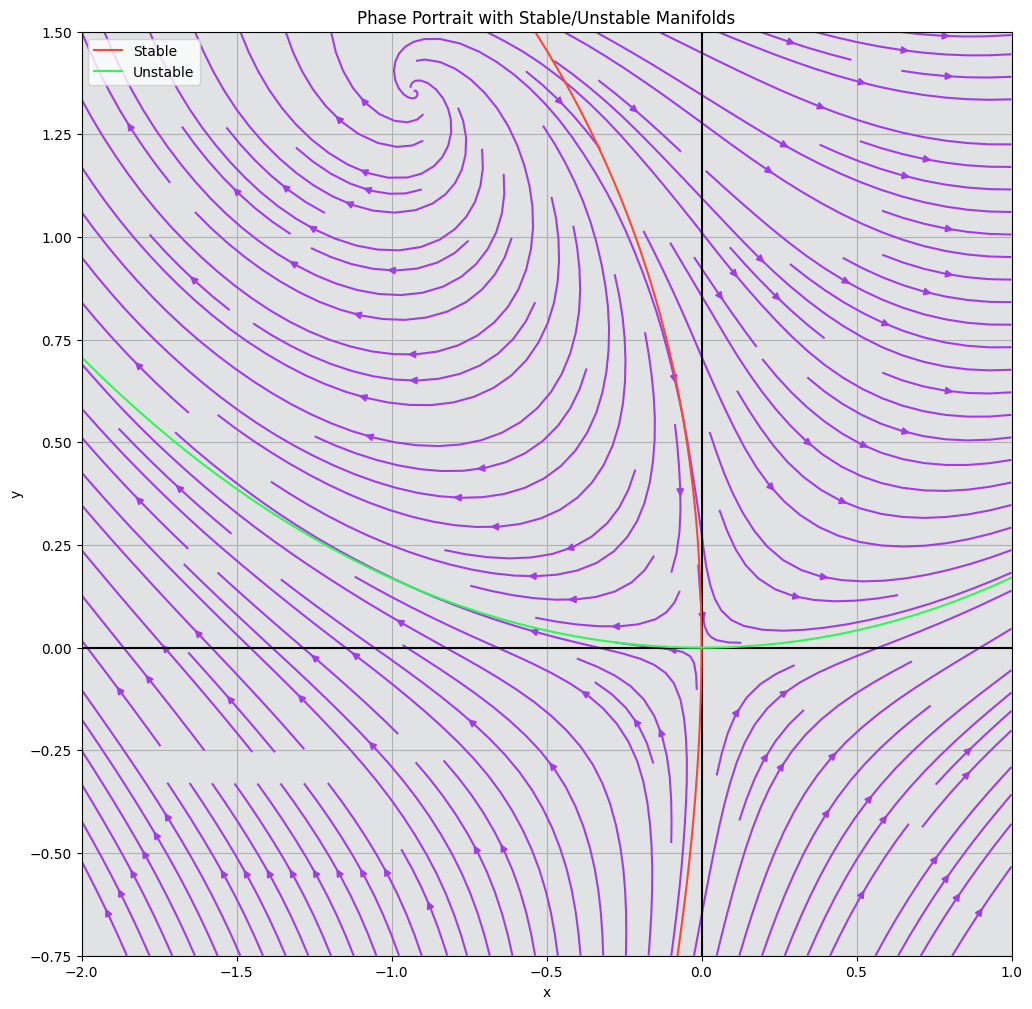
\includegraphics[width = 0.8\textwidth]{Images/Phase Portrait.png}
        \caption{Phase Portrait along with unstable and stable manifolds for the system in Problem 1.}
        \label{fig:p1a streamplot}
    \end{figure}

\clearpage
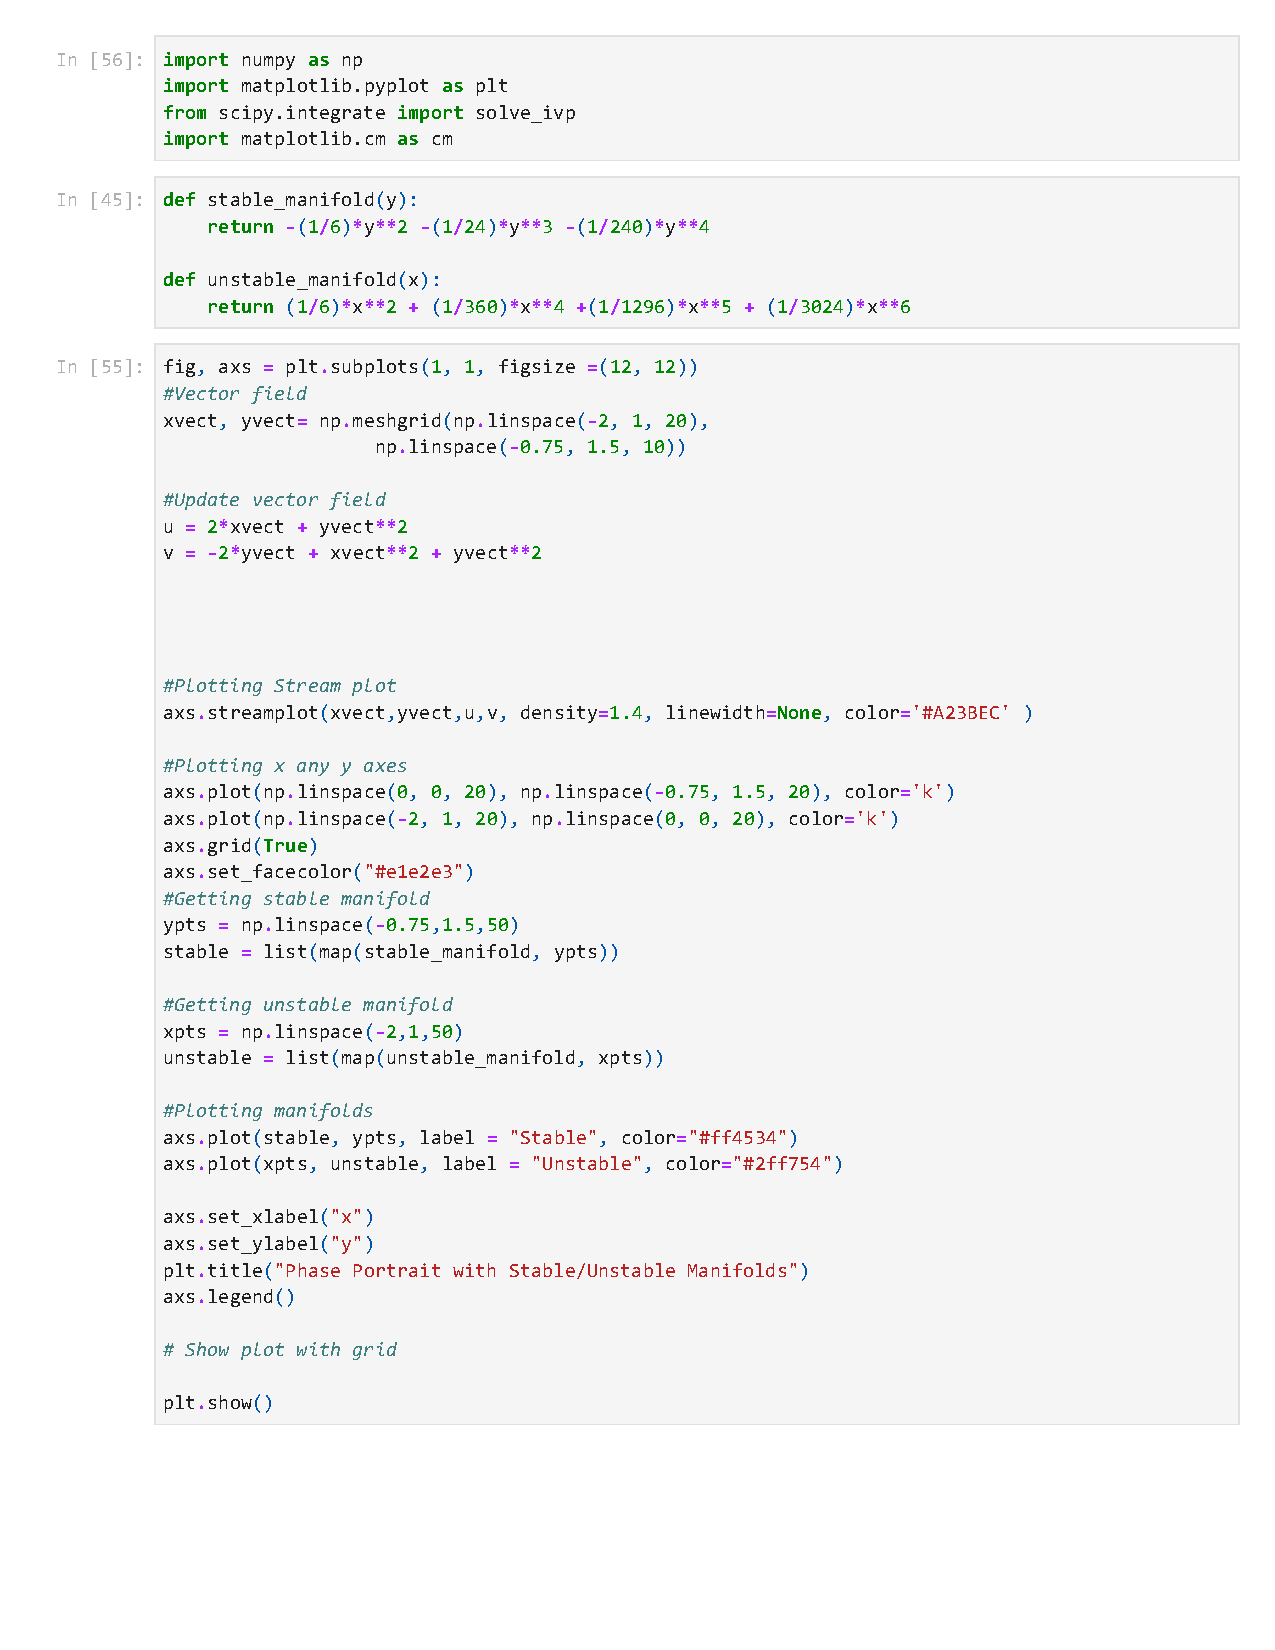
\includepdf{Code/Problem 1a.pdf}
\end{solution}

\newpage
\subsection{Problem 1, part b}
How might you use your local stable manifold to approximate a global one for this problem? How well does your approach work?
\partbreak
\begin{solution}

    One approach that I had involved stitching together the local stable manifold of all equilibrium points, but since our other equilibrium does not have a local stable manifold, we can't recover any true global stable manifold. Thus, I have come up with a far simpler idea: just take a point $(x_0, y_0)$ on our local stable manifold sufficiently close to the origin as initial conditions and run the system back in negative time. With some luck, I got it to work. I have provided my plot, where we take a point sufficiently close to our approximated equilibrium point and plot its trajectory in negative time (Here it's the yellow curve). The start and end points have been noted. It seems like the global stable manifold runs from the unstable equilibria to our saddle equilibrium. My solution seems to work perfectly fine, the problem being there is no well suited polynomial I can use to fit to this curve. This is only beneficial in a quantitative light however, so I believe this is fine. The code which plots this will follow. 

    \begin{figure}[ht]
        \centering
        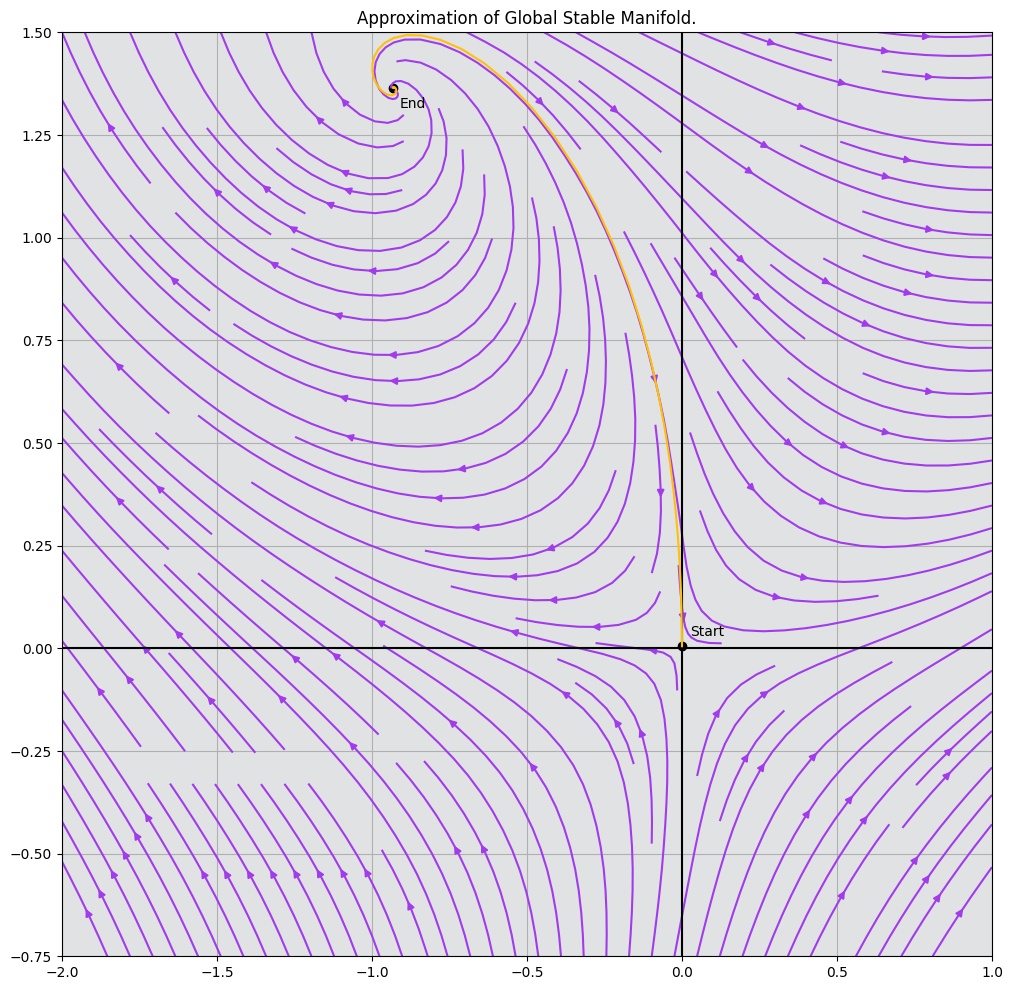
\includegraphics[width = 0.8\textwidth]{Images/Global Stable Manifold.png}
        \caption{Approximation of the Global Stable Manifold. The yellow curve begins near the origin and travels in negative time to the unstable equilibrium.}
        \label{fig:p1b GSM}
    \end{figure}

    \clearpage
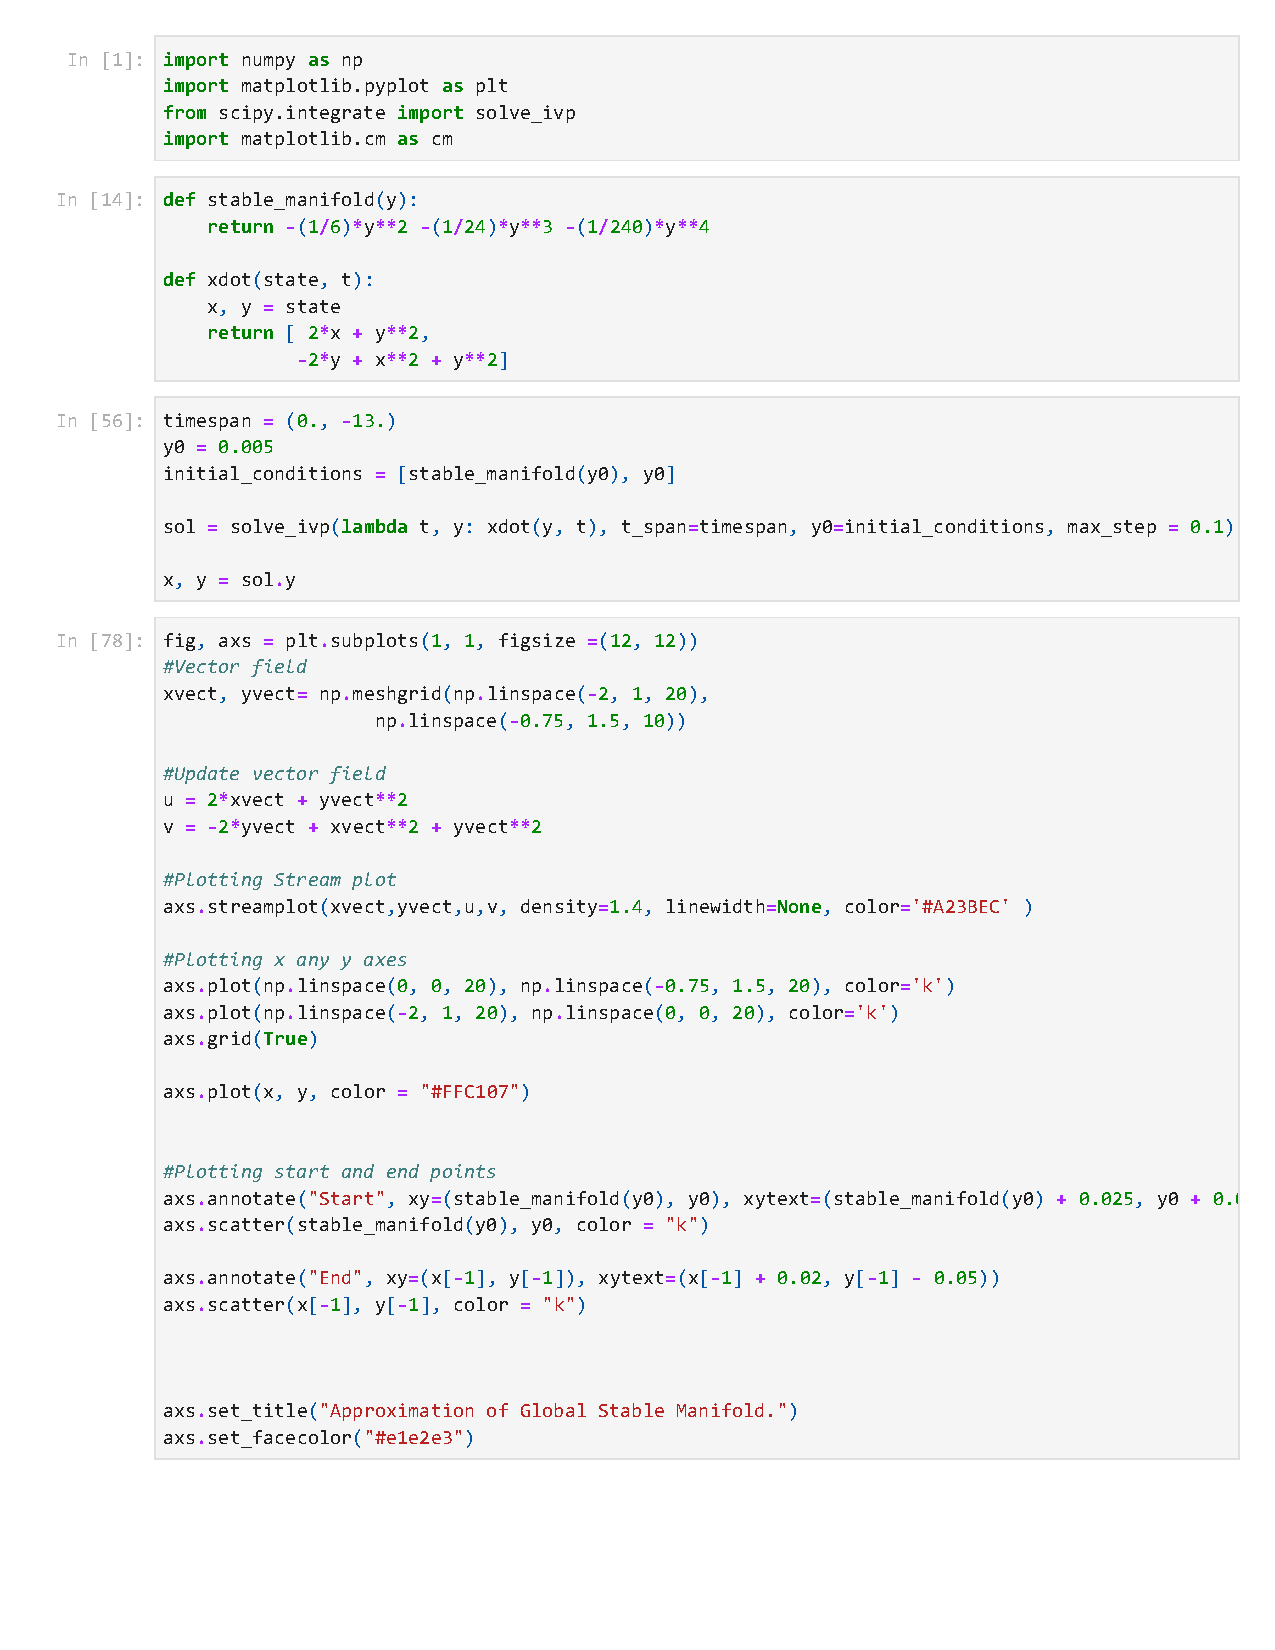
\includepdf{Code/Problem 1b.pdf}
\end{solution}

\newpage
\section{Problem 2}
Consider the following predetor-prey model:

\begin{align}
    \dot{X} &= rX\bigg(1 - \frac{c}{r}X\bigg)\bigg(\frac{X - \mu}{\nu + X}\bigg) - \bigg(\frac{\alpha XY}{\beta + X}\bigg)\label{P2: model}\\
    \dot{Y} &= \gamma \bigg( \frac{\alpha XY}{\beta + X}\bigg) - \delta Y,
    \nonumber
\end{align}
where the population densities $X, Y \geq 0$ are treated as real variables. Let $c = 0.19, \mu = 0.03, \nu = 0.003, \newline  \alpha = 800, \beta = 1.5, \gamma = 0.004, \delta = 2.2$. We will explore what happens when we vary $r \in (0, 3).$

\subsection{Problem 2, part a}
First, which variable, $X$ or $Y$, represents the predator population and which represents the prey population? This model incorporates a ``strong Allee effect". What is that? what term encodes it?
\partbreak
\begin{solution}

    It seems as though the prey population is represented here as $X(t)$, while the predator population is represented as $Y(T)$. This is only inferred from reading online about predator-prey models. The ``strong Allee effect" refers to there being a critical population point where, once it is hit, the species is doomed to extinction without any external forces. I have included a plot which represents this phenomena, taken from the Wikipedia page for the Allee Effect. Furthermore, it seems upon further reading \cite{ye2019dynamic}, the Allee Effect is encoded in the $\mu$ variable.

\begin{figure}[ht]
    \centering
    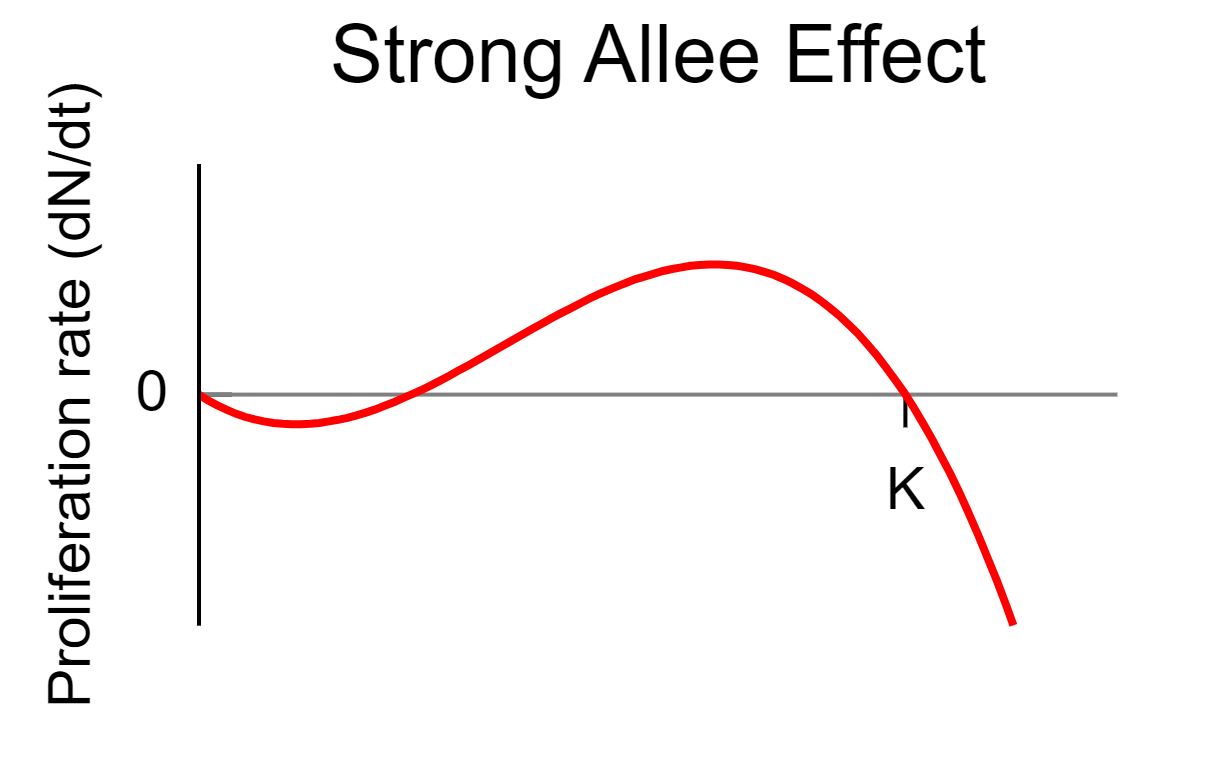
\includegraphics[width = 0.6\textwidth, frame]{Images/Strong Allee Effect.png}
    \caption{Strong Allee Effect. The critical point is denoted $K$. Once this has been breached from the left, there is no hope for the species.}
    \label{fig:p2a strong allee effect}
\end{figure}
\end{solution}

\newpage
\subsection{Problem 2, part b}
Show that there are 3 equilibrium solutions for $r < r_0$ and four for $r > r_0$ where you determine the values for $r_0$. In the phase plane, a periodic orbit must enclose at least one fixed point, according to Corollary 6.26 in Section 6.5 of Meiss. Use this, together with the dynamical invariance of the $X$ and $Y$ axes, to argue that there are no periodic solutions for $r \leq r_0$.
\partbreak
\begin{solution}

    Note for equilibrium solutions, we require $f(\textbf{x}) = 0$, where $f(\textbf{x})$ is the right hand side of (\ref{P2: model}). Then, the we notice:
    \begin{align*}
        0&= \gamma \bigg( \frac{\alpha xy}{\beta + x}\bigg) - \delta y &\text{(Second equation.)}\\
       0 &= y\Bigg(\frac{\gamma \alpha x}{\beta + x} - \delta\Bigg) &\text{(Grouping.)}
    \end{align*}
    which will create two separate cases. 
    \hrule
    \begin{enumerate}
        \item \underline{Case 1:} $y = 0$

        Then by the first equation:
        \tightalignbreak
        \begin{align*}
            0 &=(rx - cx^2)\bigg(\frac{x - \mu}{\nu + x}\bigg)\\
            0 &= (rx - cx^2)(x - \mu) &(\nu + x > 0.)\\
            \implies 0 &= x(r - cx)(x - \mu) &\text{(Factoring.)}
        \end{align*}
        \alignbreak
        Therefore, this will permit three equilibrium solutions, namely at $(0, 0), (\frac{r}{c}, 0), (\mu, 0)$.
        \newpage
        \item \underline{Case 2:} $\frac{\gamma \alpha x}{\beta + x} - \delta = 0$

        After rearranging, this gives $x = \frac{\delta \beta}{\gamma\alpha - \delta}$. Note that, since our parameters are fixed, we notice that $\gamma\alpha - \delta = 1$. So $x$ can be simplified to just $x = \delta \beta = 3.3$. If we plug this into the first equation, we can find what $y$ must then equal.
        \tightalignbreak
        \begin{align*}
            0&= r\delta\beta(1 - \frac{c}{r}\delta\beta)\bigg(\frac{\delta \beta - \mu}{\nu + \delta\beta}\bigg) - \frac{\alpha\delta\beta y}{\beta(1 + \delta)} &\text{(After simplification.)}\\
            &= \delta\beta(r - c\beta\delta)\bigg(\frac{\delta \beta - \mu}{\nu + \delta\beta}\bigg) - \frac{\alpha\delta\beta y}{\beta\gamma\alpha} &(\gamma\alpha - \delta = 1.)\\
            &= \delta\beta(r - c\beta\delta)\bigg(\frac{\delta \beta - \mu}{\nu + \delta\beta}\bigg) - \frac{\delta y}{\gamma} &\text{(Simplifying.)}\\
            \implies y &= \gamma\beta(r - c\delta\beta)\bigg(\frac{\delta \beta - \mu}{\nu + \delta\beta}\bigg) &\text{(Solving for $y$.)}
        \end{align*}
        \alignbreak
        Since $y \geq 0$, this would imply $r \geq c\delta \beta$. Therefore $r_0 = c\delta \beta = 0.627$. Therefore, our fourth equilibrium point, at
        \[
        (x, y) = (\beta\delta, \gamma\beta(r - c\delta\beta)\bigg(\frac{\delta \beta - \mu}{\nu + \delta\beta}\bigg))
        \]
        is allowed only for $r > c\delta \beta$. If $r = c\delta\beta$, then our second equilibrium point found in case 1 would coincide with this one. 
    \end{enumerate}
    \hrule

    \jump
    Therefore we have shown there are three equilibrium, $(0, 0), (\frac{r}{c}, 0), (\mu, 0)$ for $r < r_0$, and an additional one which appears for $r > r_0$. Corollary 6.26 concisely states ``Any periodic orbit of f must enclose at least one equilibrium." The only equilibrium which could possibly be enclosed by a periodic orbit is the one given off the boundary (due to our restriction $X, Y \geq 0$), which is only allowed for $r > r_0$. Therefore, no periodic orbits exist for $r \leq r_0$.
\end{solution}

\newpage
\subsection{Problem 2, part c}
The interval of $r$ that admits limit cycles is $r \in (r_H, r_h)$; one end of the interval is associated with a Hopf bifurcation $r_H$ and the other with a heteroclinic orbit, $r_h$. Estimate both $r_H$ and $r_h$ numerically, and also plot the period of the oscillations as a function of $r$ on the interval between $r_H$ and $r_h$. 
\partbreak
\begin{solution}

    The Hopf bifurcation will happen when orbits which previously limits to the stable equilibrium no longer do so, favoring a nonzero periodic orbit. The heteroclinic bifurcation will happen when an orbit intersects a saddle point, abruptly ending the orbit. We can numerically find the $r$ values which permit this behavior numerically. After choosing a random initial condition and observing its orbit for various values, I find that the Hopf bifurcation happens at around $ r_H = 1.46$ and the heteroclinic bifurcation at $r_h = 2.65$. The predator and prey population densities are recorded for $5$ different values of $r \in (r_H, r_h)$ in Figure \ref{fig:p2c orbits}. After this, we can investigate the timesteps taken to get to the next max of the populations, as shown in Figure \ref{fig:p2c Period timings}. Then, we investigate the divergence of these timings in Figure \ref{fig:p2c Period div}. Note that the timestep is not a general notion of time, it is just the step taken in the ode solver I used. The code to generate each plot follows their respective plot.

    \begin{figure}
        \centering
        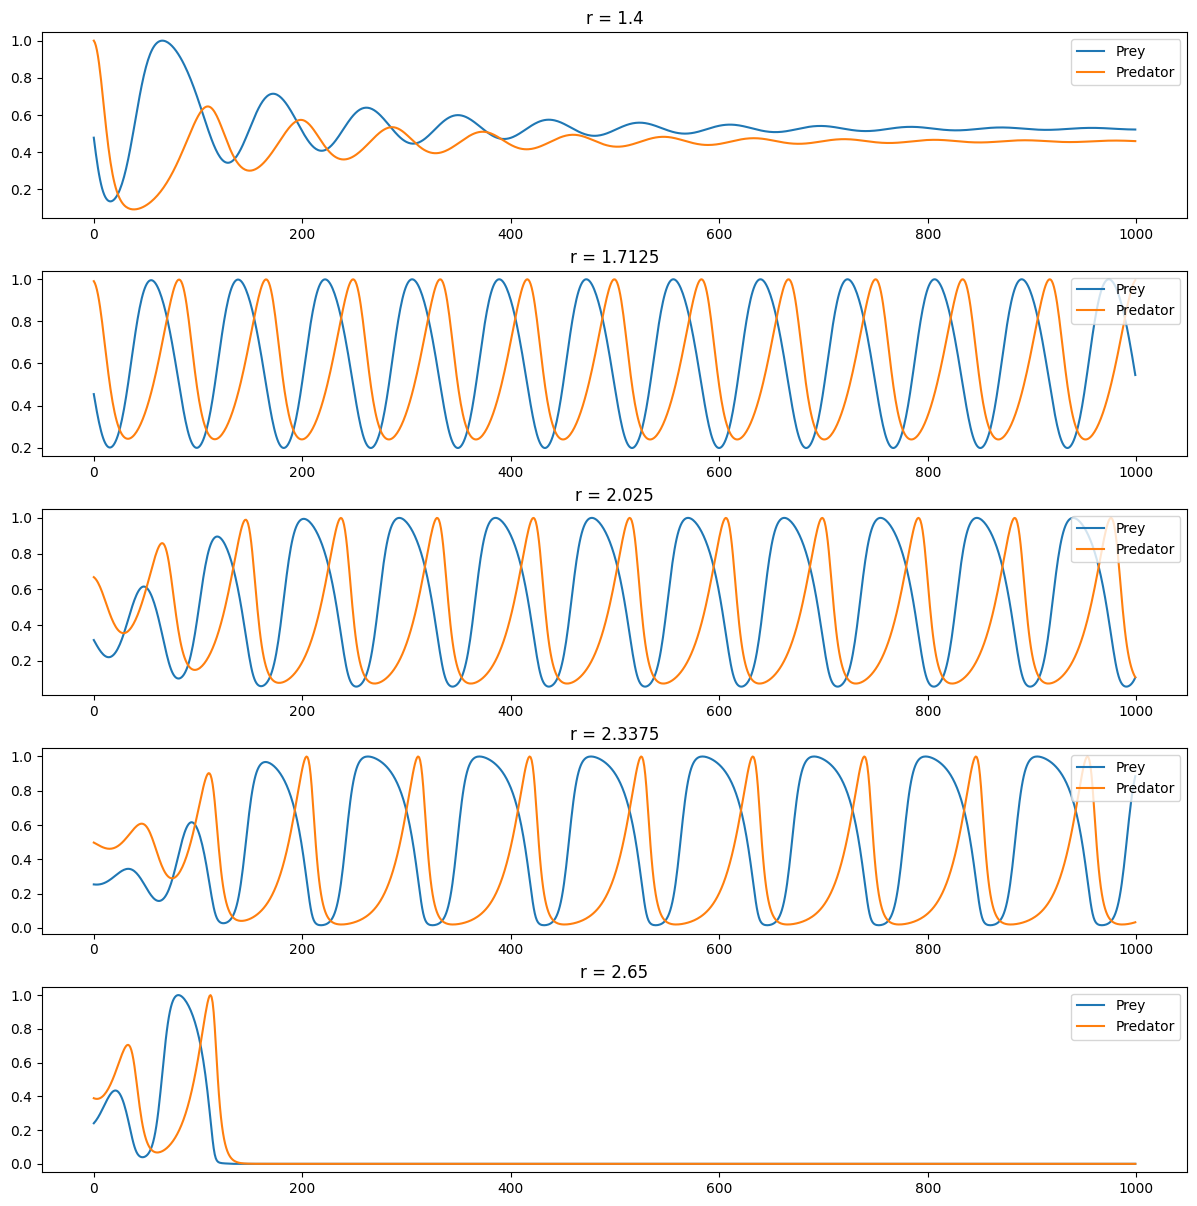
\includegraphics[width = 0.8\textwidth]{Images/Orbits for different r.png}
        \caption{Orbits for various values of $r \in (r_H, r_h)$. Note the populations collapse st some finite time for $r = 2.65$, while the populations limit to the equilibrium for $r = 1.4.$}
        \label{fig:p2c orbits}
    \end{figure}

    \clearpage
    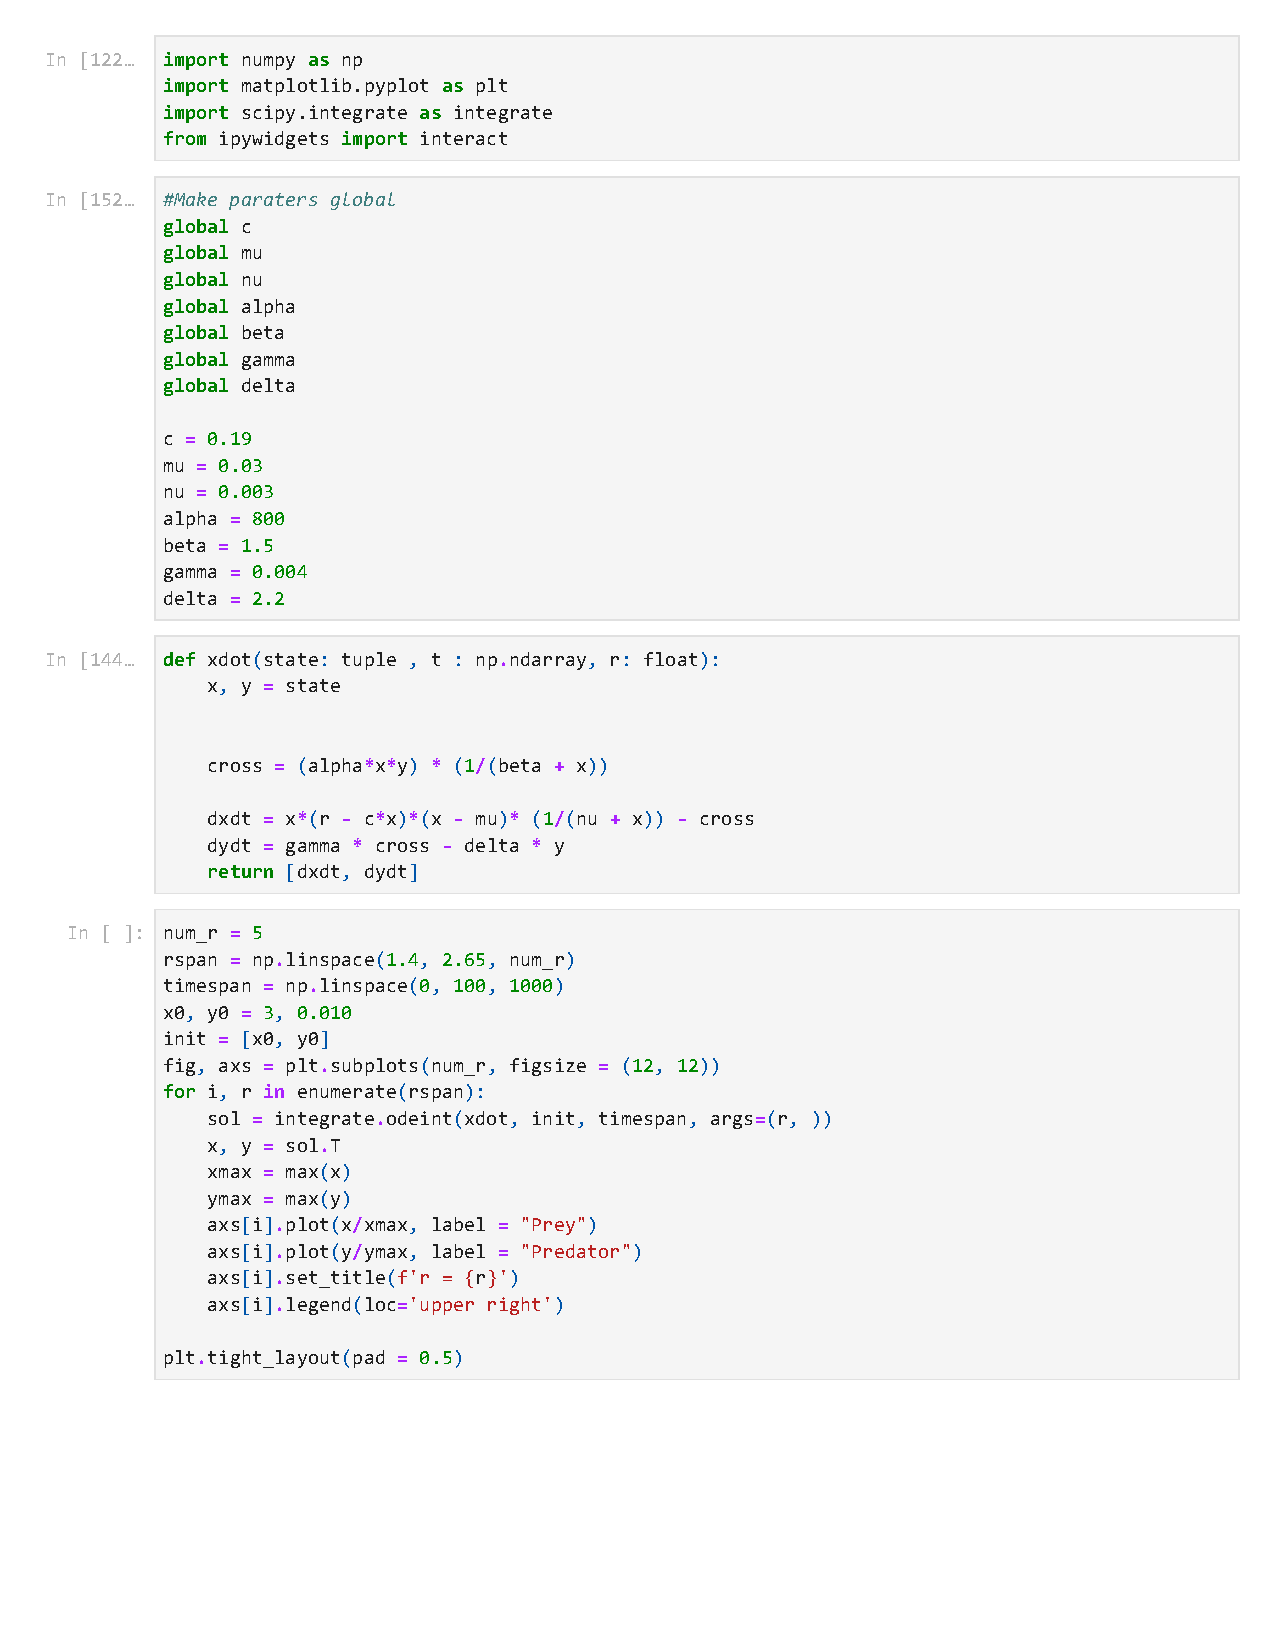
\includepdf{Code/Problem 2c.pdf}

    \begin{figure}
        \centering
        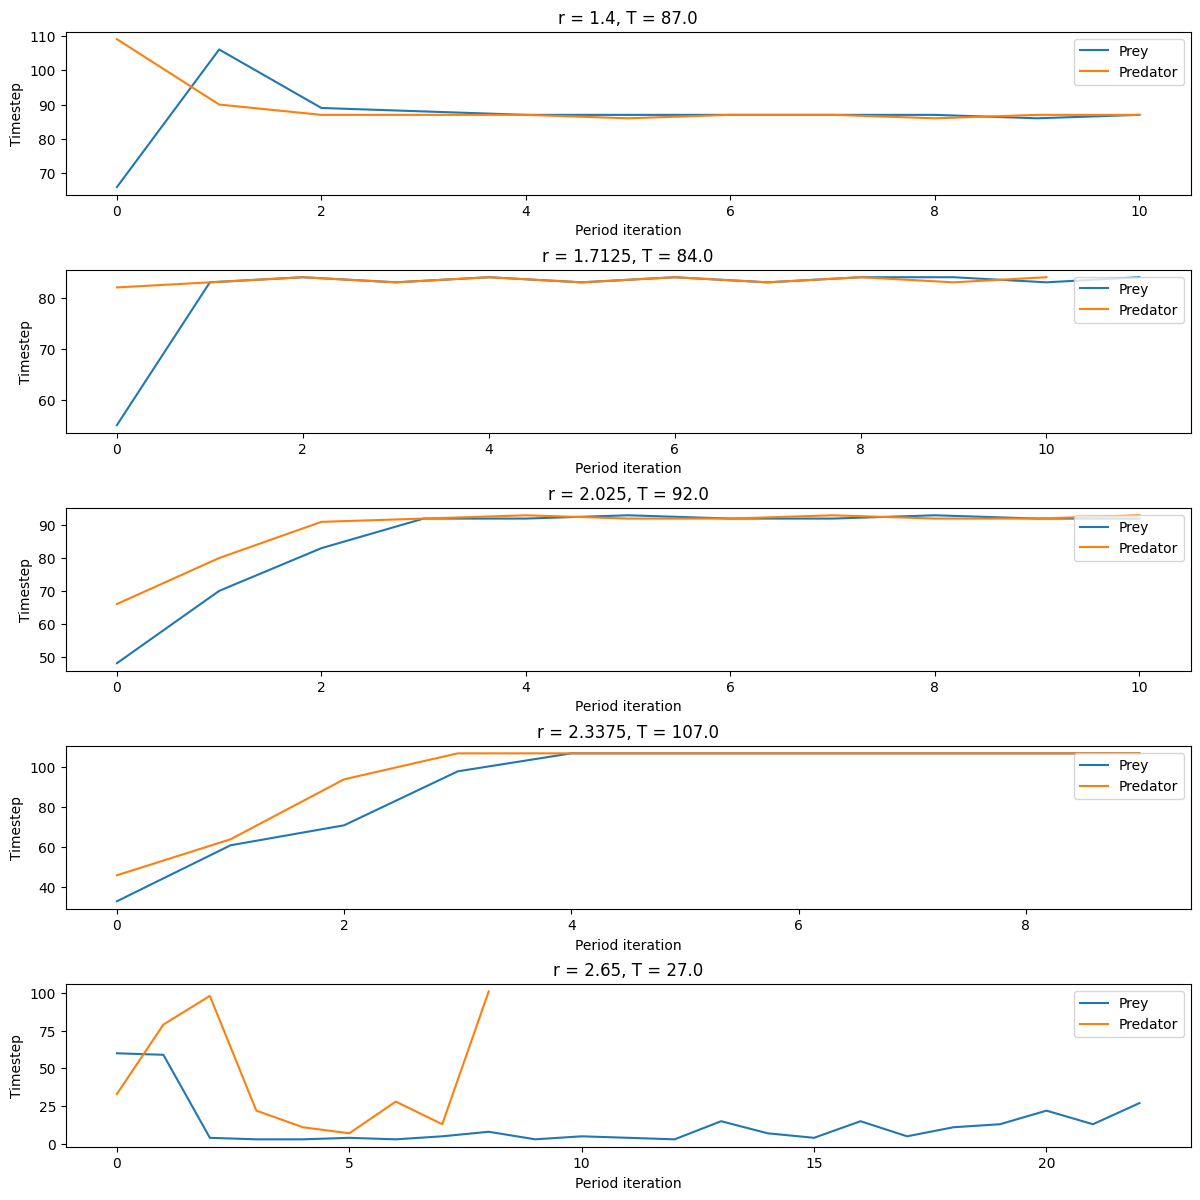
\includegraphics[width = 0.8\textwidth]{Images/Period timings.png}
        \caption{The timesteps between max size populations for Predator and Prey. The ``limit period" is given in the title. The last plot can be safely ignored, since the entries zero out after the first three.}
        \label{fig:p2c Period timings}
    \end{figure}
    \clearpage
    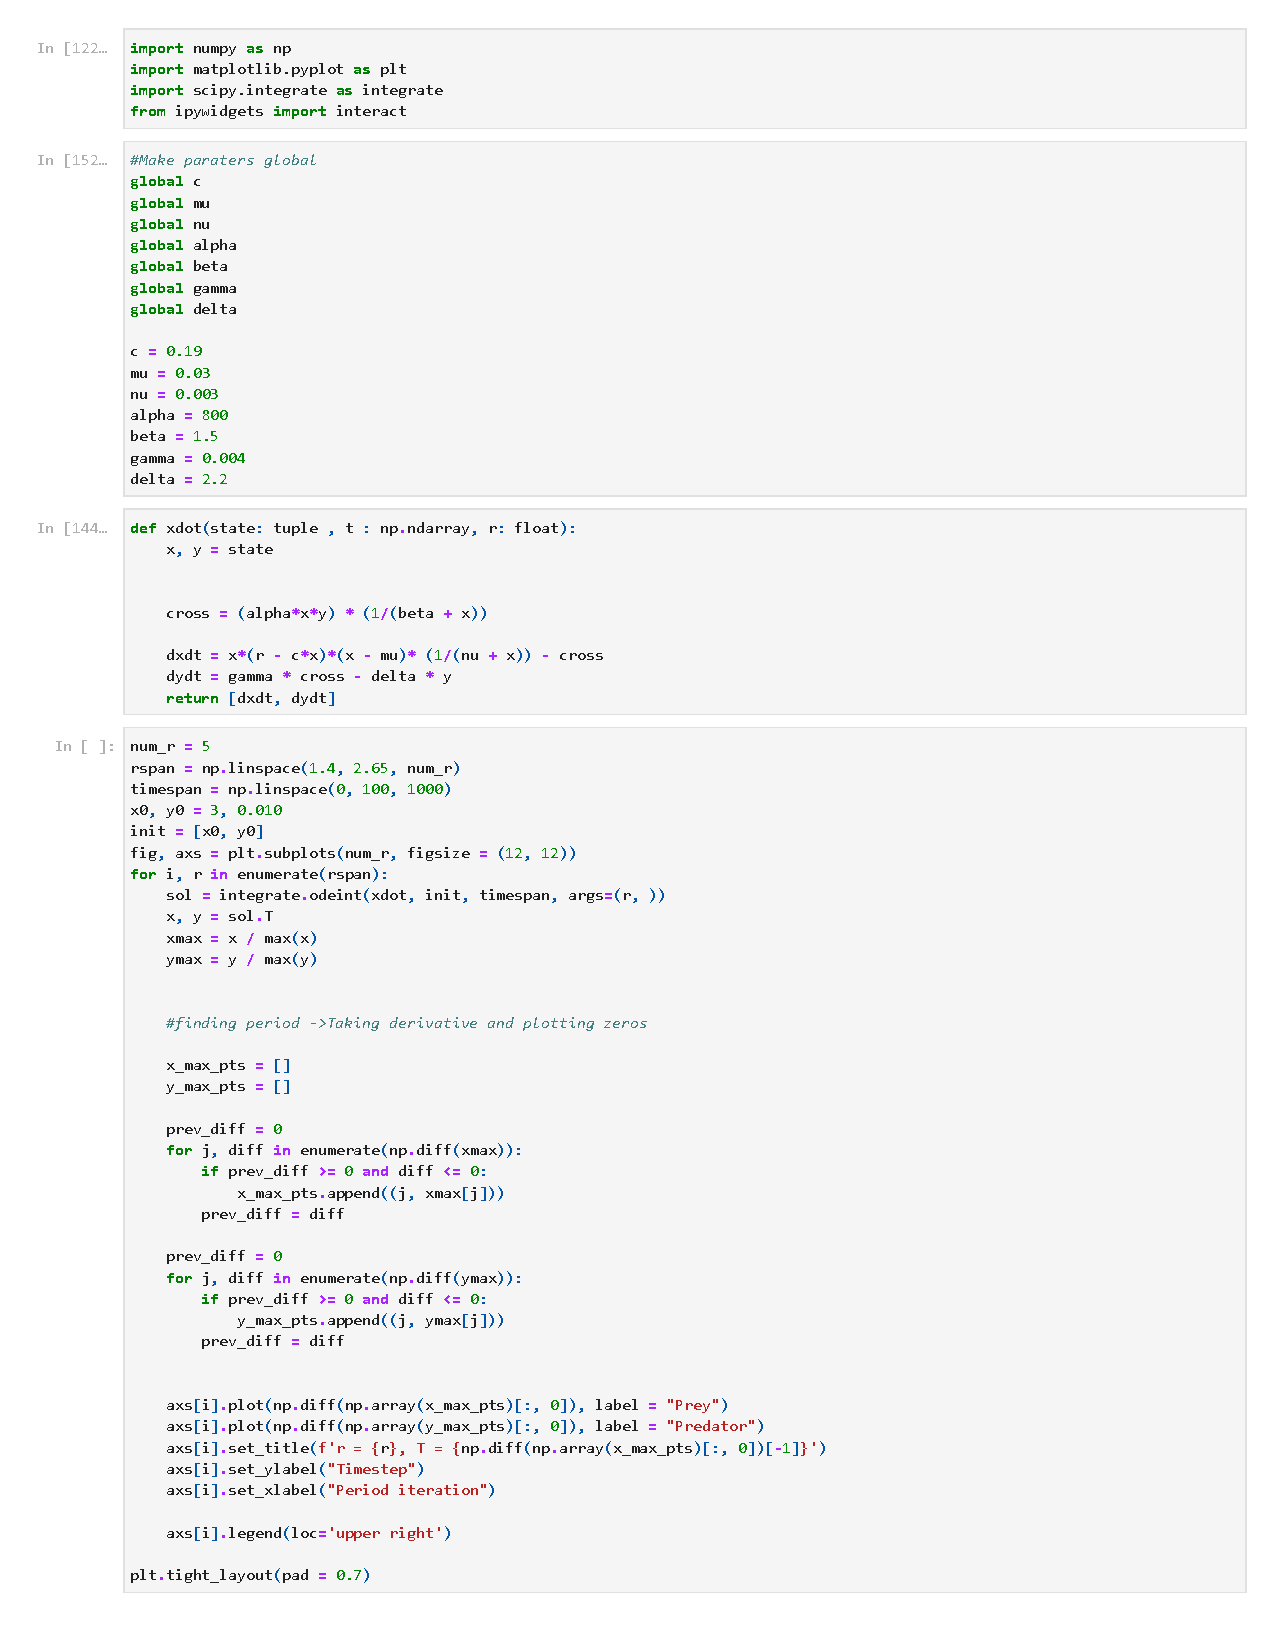
\includepdf{Code/Problem 2c2.pdf}

    \begin{figure}
        \centering
        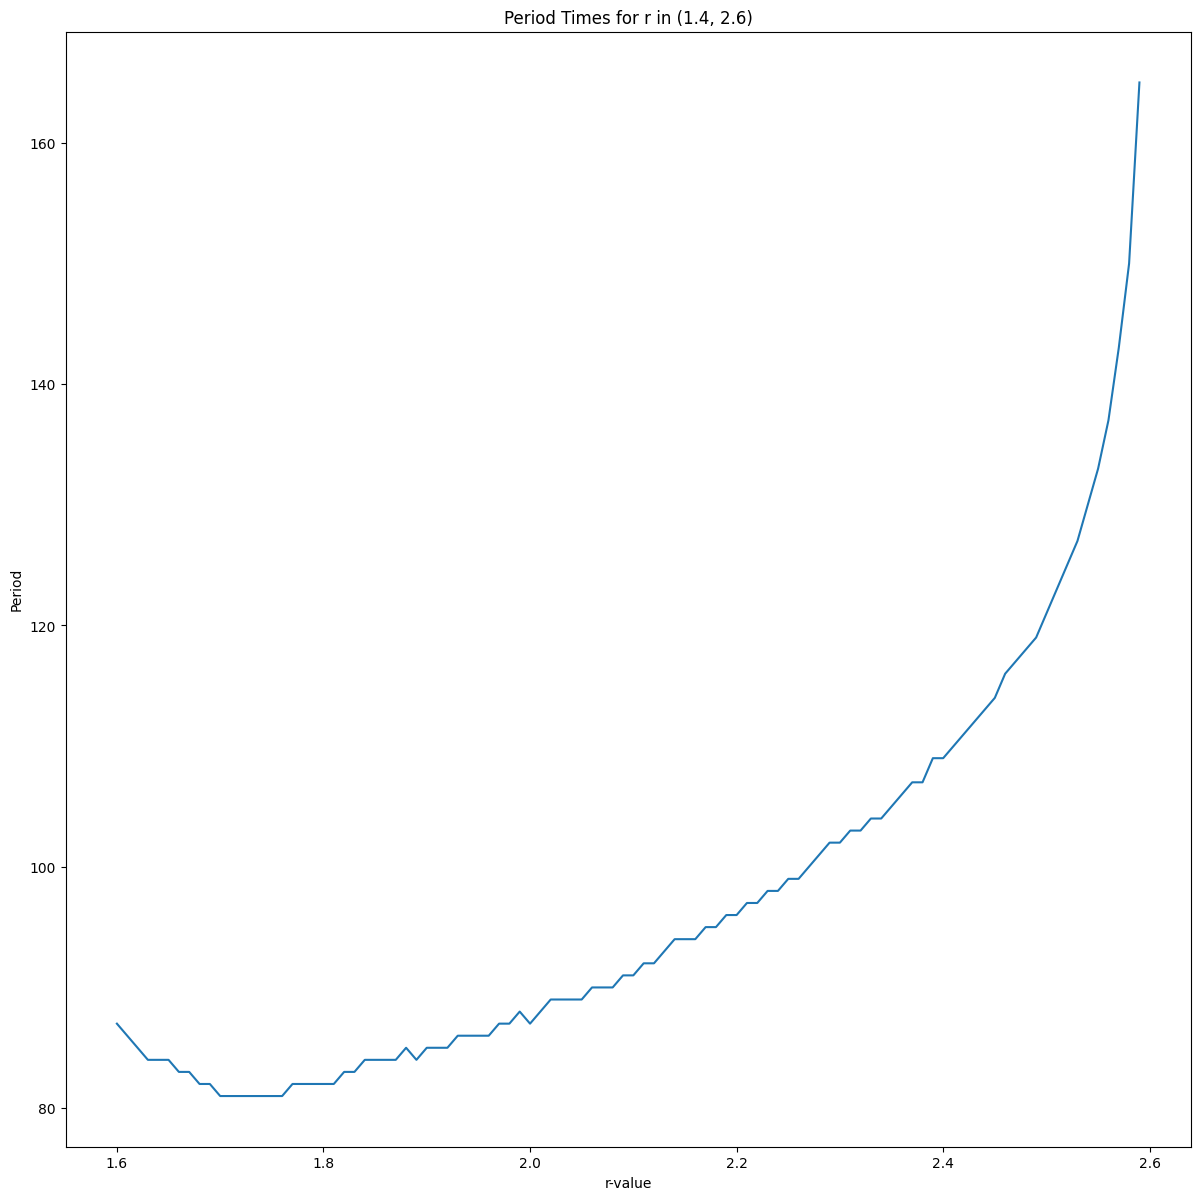
\includegraphics[width = 0.8\textwidth]{Images/Period Divergance.png}
        \caption{Period times for $r \in (r_H, r_h)$. Note the period seems to diverge when $r \rightarrow r_h$.}
        \label{fig:p2c Period div}
    \end{figure}

    \clearpage
    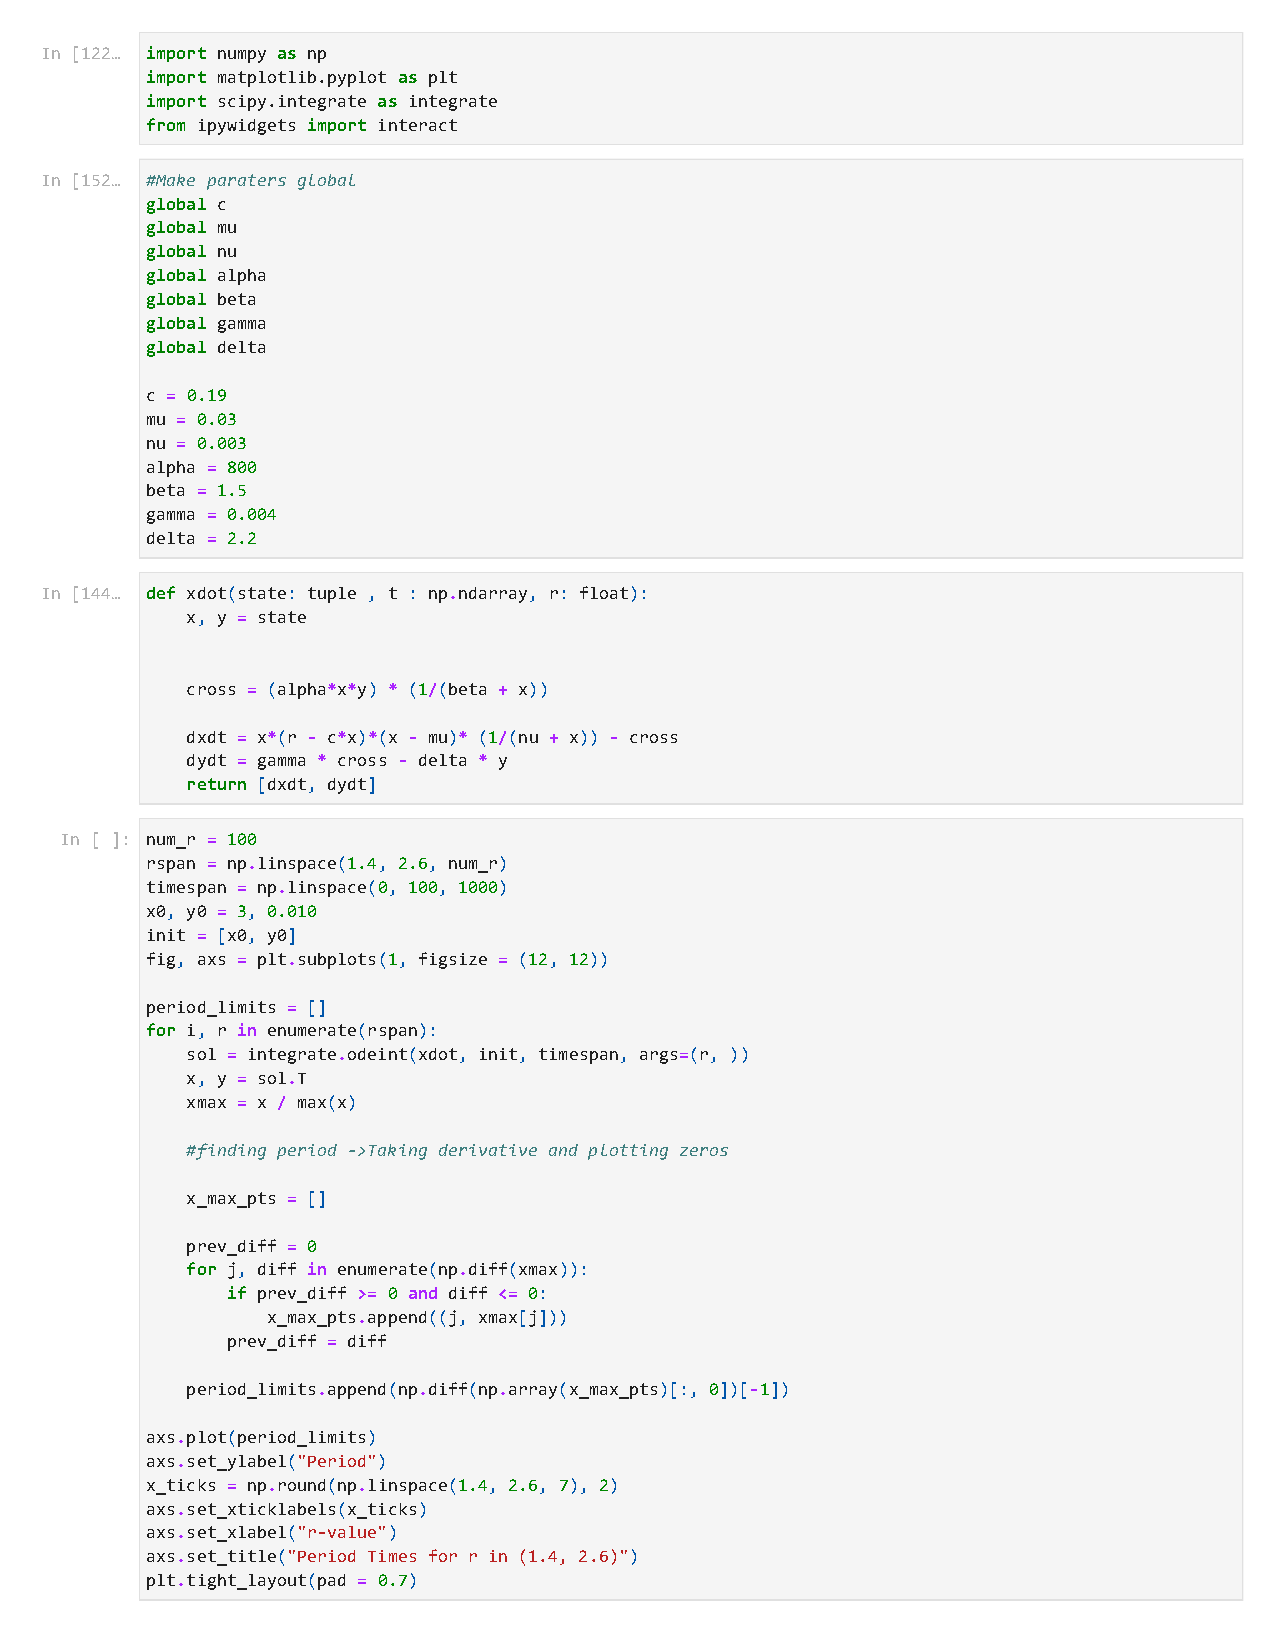
\includepdf{Code/Problem 2c3.pdf}
\end{solution}

\newpage
\subsection{Problem 2, part d}
For the $r$ parameter range $r \in (r_H, r_h)$, estimate the Floquet multiplier associated with the limit cycle $\mu(r)$. 
\partbreak
\begin{solution}

    Do the same analysis again to get the limit period of a limit cycle, for r in that range. Then integrate the trace of the Jacobian of the system evaluated at x(t), y(t) along one period to get the determinant of the fundamental matrix (Abel's theorem). 
\end{solution}
\newpage
\section{Problem 3}
This problem relates to some parts of the proof of Theorem 5.9 (Local Stable Manifold) in the textbook. For full credit on this problem, you need to concisely summarize the relevant parts of the proof in your answer.  

\subsection{Problem 3, part a}
The proof relies on the contraction mapping theorem. Explain its role in the proof. What is the mapping? What is the origin of the three terms in $T(x)(t)$ given by equation 5.17? What is the bound on the contraction rate $c$ obtained in the proof, and how do we ensure $c < 1$?
\partbreak
\begin{solution}

    The contraction mapping theorem, as well as its generalization (Theorem 5.11, the Uniform Contraction Principle) are applied within the first and third parts of the proof respectively. I will explain the role of the contraction mapping theorem - and not its generalization- here, since it was not explicitly mentioned. The contraction mapping theorem will imply that, once we show the mapping 
    \[
    T(x)(t) = e^{tA}\sigma + \int_0^t e^{(t - s)}\pi_sg(x(s))ds - \int_t^\infty e^{(t - s)A}\pi_ug(x(s))ds
    \]
    is indeed a contraction mapping, then we are guaranteed to have a unique fixed point in our set $V_\delta$, defined as
    \[
    V_\delta = \{ x \in C^0(\R^+, \R^n): \norm{x} \leq \delta\}.
    \]
    This gives justification to the fact that the unique solution $x(t;\sigma)$ evaluated at $t = 0$ is a graph over our stable eigenspace, $E^s$. This mapping is generated by evaluating projections of the general solution to the affine, nonautonomous initial value problem (5.12), given as
    \[
    x(t) = e^{(t - \tau)A}x(\tau) + \int_\tau^t e^{(t - s)A}\gamma(s)ds,
    \]
    for some initial condition $x(\tau)$ given at some arbitrary time $t = \tau$. This is presented as Lemma 5.8 in the text. Note that, evaluating $\tau = 0$ and $x(0) = \sigma \in E^s$, then we recover the first and second term in the mapping. The third term is similarly found by projection the general solution onto the unstable eigenspace, $E^u$ of A. 

    \jump
    The constant $c$ arises for $T$ being a uniform contraction. This constant will be restricted to the interval $(0, 1)$, however a tighter lower bound is found in Exercise 6, giving $\norm{D_xT} \leq c$ as a result. Note $D_xT$ is the partial derivative of T with respect to x. Furthermore, we can ensure $c < 1$ due to the mapping $T$ being a uniform contraction mapping, thus having Lipschitz constant $< 1$. Note that $c$ is the Lipschitz constant for $T$.
\end{solution}

\newpage
\subsection{Problem 3, part b}
Show that any bounded fixed point of the map defined by (5.17) solves the differential equation (5.10).
\partbreak
\begin{solution}

Note the map in (5.17) refers to 
\[
T(x)(t) = e^{tA}\sigma + \int_0^t e^{(t - s)A}\pi_sg(x(s))ds - \int_t^\infty e^{(t - s)A}\pi_ug(x(s))ds.
\]
Moreover the differential equation in (5.10) is the given as
\[
\xdot = Ax + g(x),
\]
where $g(x) = f(x - x^*) - Ax$ is given as the nonlinear terms in the equation, so $g(0) = 0$ and $Dg(0) = 0$. If $x$ is a fixed point of the mapping, then applying $T$ to $x$ will just return $x$. That is, $x = T(x)$. Differentiating both sides with respect to $t$ then gives the following:

\alignbreak
{\footnotesize
\begin{align*}
    \frac{d}{dt}T(x)(t) &= \frac{d}{dt}\Bigg[ e^{tA}\sigma + \int_0^t e^{(t - s)A}\pi_sg(x(s))ds - \int_t^\infty e^{(t - s)A}\pi_ug(x(s))ds\Bigg] &\text{(Given.)}\\
    &= \frac{d}{dt}e^{tA}\sigma + \frac{d}{dt}\int_0^t e^{(t - s)A}\pi_sg(x(s))ds - \frac{d}{dt}\int_t^\infty e^{(t - s)A}\pi_ug(x(s))ds &\text{(Linearity.)}\\
    &= Ae^{tA}\sigma + \frac{d}{dt}\int_0^t e^{(t - s)A}\pi_sg(x(s))ds - \frac{d}{dt}\int_t^\infty e^{(t - s)A}\pi_ug(x(s))ds &\text{(First term.)}\\
    &= Ae^{tA}\sigma + \pi_sg(x(t)) + \pi_ug(x(t))\int_0^t \frac{\partial}{\partial t}e^{(t - s)A}\pi_sg(x(s))ds - \int_t^\infty \frac{\partial}{\partial t}e^{(t - s)A}\pi_ug(x(s))ds &\text{(Leibnitz rule.)}\\
    &= Ae^{tA}\sigma + \pi_sg(x(t)) + \pi_ug(x(t))\int_0^t Ae^{(t - s)A}\pi_sg(x(s))ds - \int_t^\infty Ae^{(t - s)A}\pi_ug(x(s))ds &\text{(Differentiation.)}\\
    &= A\Bigg(e^{tA}\sigma \int_0^t Ae^{(t - s)A}\pi_sg(x(s))ds - \int_t^\infty Ae^{(t - s)A}\pi_ug(x(s))ds \Bigg) + \pi_sg(x(t)) + \pi_ug(x(t)) &\text{{(Grouping.)}}\\
    &=  A\Bigg(e^{tA}\sigma \int_0^t Ae^{(t - s)A}\pi_sg(x(s))ds - \int_t^\infty Ae^{(t - s)A}\pi_ug(x(s))ds \Bigg) + g(x(t)) &\text{(Direct sum.)}\\
    &= AT(x) + g(x(t)) &\text{(T definition.)}\\
    &= Ax + g(x(t)) &(Tx = x.)
\end{align*}
\alignbreak
}
\end{solution}


\newpage
\subsection{Problem 3, part c}
The proof also uses a Gr\"onwall's inequality. What is its role in the proof?
\partbreak
\begin{solution}

    The Gr\"onwall's inequality used in the proof of the generalized one given in Chapter 3. It is used in part 2 in the proof to show that our unique fixed point solution $x(t;\sigma)$ is a point on the stable manifold. That is, $|x(t;\sigma)| \rightarrow 0$ as $t \rightarrow \infty$. As a means for clarity, I will provide Lemma 5.10 (Generalized Gr\"onwall) here, but omit its proof. 
    \begin{center}\rule{0.89\textwidth}{.4pt}\end{center}
    \vspace{-8mm}
    \begin{quote}
    $\textbf{Lemma 5.10 (Generalized Gr\"onwall)}.$ Suppose $\alpha, M$ and $L$ are nonnegative, $L <\alpha /2$, and there is a nonnegative bounded continuous function $u: \R^+ \rightarrow \R^+$ satisfying
    \[
    u(t) \leq e^{-\alpha t}M + L\int_0^te^{-\alpha(t - s)}u(s)ds + L\int_t^\infty e^{\alpha(t - s)}u(s)ds;
    \]
    then $u(t) \leq \frac{M}{\beta} e^{-(\alpha - L/\beta)t}$, where $\beta = 1 - 2\frac{L}{\alpha}$.
    \end{quote}
    \vspace{-10mm}
    \begin{center}\rule{0.89\textwidth}{.4pt}\end{center}
    \jump
    
    Once the inequality is proven we get the following bound for $x(t;\sigma)$:

    \[
    \abs{x(t;\sigma)} \leq 2Ke^{-\alpha t/2}\abs{\sigma},
    \]
    which directly implies that $x(t; \sigma)$ belongs to the stable manifold for all $\sigma \in E^s.$
\end{solution}
\newpage
\printbibliography
\end{document}